\documentclass[10pt]{article}
\usepackage[margin=0.72in]{geometry}
\usepackage{graphicx,array,hyperref,caption,titlesec,fancyhdr}
\hypersetup{colorlinks=true,urlcolor=black,linkcolor=black,citecolor=black}
\setlength{\parindent}{0pt}
\setlength{\parskip}{4pt}
\captionsetup{font=small,labelfont=it,textfont=it}
\titleformat{\section}{\large\bfseries}{}{0pt}{}
\titlespacing*{\section}{0pt}{7pt}{3pt}
\pagestyle{fancy}
\fancyhf{}
\lfoot{CS740 Project -- Eigenfaces vs. Fisherfaces}
\rfoot{Page \thepage}
\renewcommand{\headrulewidth}{0pt}
\renewcommand{\footrulewidth}{0.4pt}
\begin{document}

\begin{center}
{\LARGE\bfseries Eigenfaces versus Fisherfaces\par}
\vspace{3pt}
{\large Face Recognition Using Class-Specific Linear Projection\par}
\vspace{4pt}
{\normalsize Yashwanth Sudi (26M0794)\par}
\end{center}

\section{1. Introduction}
This project implements the face-recognition methods in Belhumeur, Hespanha, and Kriegman (1997) and evaluates them on the ORL and Extended Yale B datasets. Both methods first represent a face image as a vector and then use nearest-neighbor recognition in a lower-dimensional feature space.

\textbf{Eigenfaces (PCA)} learns the directions with maximum overall image variance. It is unsupervised, so subject labels are not used when learning the projection. \textbf{Fisherfaces (PCA + FLD)} first reduces the high-dimensional image space with PCA and then applies Fisher Linear Discriminant (FLD). FLD uses subject labels to maximize between-person variation while minimizing within-person variation.

For both methods, Euclidean and correlation distance were evaluated. The ORL split uses the first 32 subjects. Yale uses all readable subject folders; three truncated PGM files were ignored by the image reader.

\section{2. Experimental Results}
The table compares the final, largest-gallery setting for each dataset. The ``best metric'' is the higher of Euclidean and correlation matching for that method.

\begin{center}
\small\renewcommand{\arraystretch}{1.25}
\begin{tabular}{|>{\centering\arraybackslash}p{1.35in}|>{\centering\arraybackslash}p{1.15in}|>{\centering\arraybackslash}p{1.15in}|p{2.45in}|}
\hline
\textbf{Dataset / gallery} & \textbf{Eigenfaces best} & \textbf{Fisherfaces best} & \centering\textbf{Main observation}\arraybackslash \\
\hline
ORL / 6 images per subject & 95.31\% (Correlation) & 94.53\% (Correlation) & Both methods are strong; PCA is marginally higher. \\
\hline
Yale / 40 images per subject & 35.64\% (Euclidean) & 77.88\% (Correlation) & Fisherfaces improves accuracy by 42.23 points. \\
\hline
\end{tabular}
\captionof{table}{Recognition accuracy in the largest gallery experiment.}
\end{center}

ORL contains relatively controlled images, so both representations reach about 95\% accuracy. Yale has large lighting changes; the Fisherfaces result is substantially better because the discriminant projection suppresses illumination-related within-class variation. Correlation matching is particularly effective for Fisherfaces on Yale.

\section{3. Accuracy versus Retained Dimensions}
\begin{figure}[h!]
\centering
\begin{minipage}[t]{0.48\textwidth}\centering
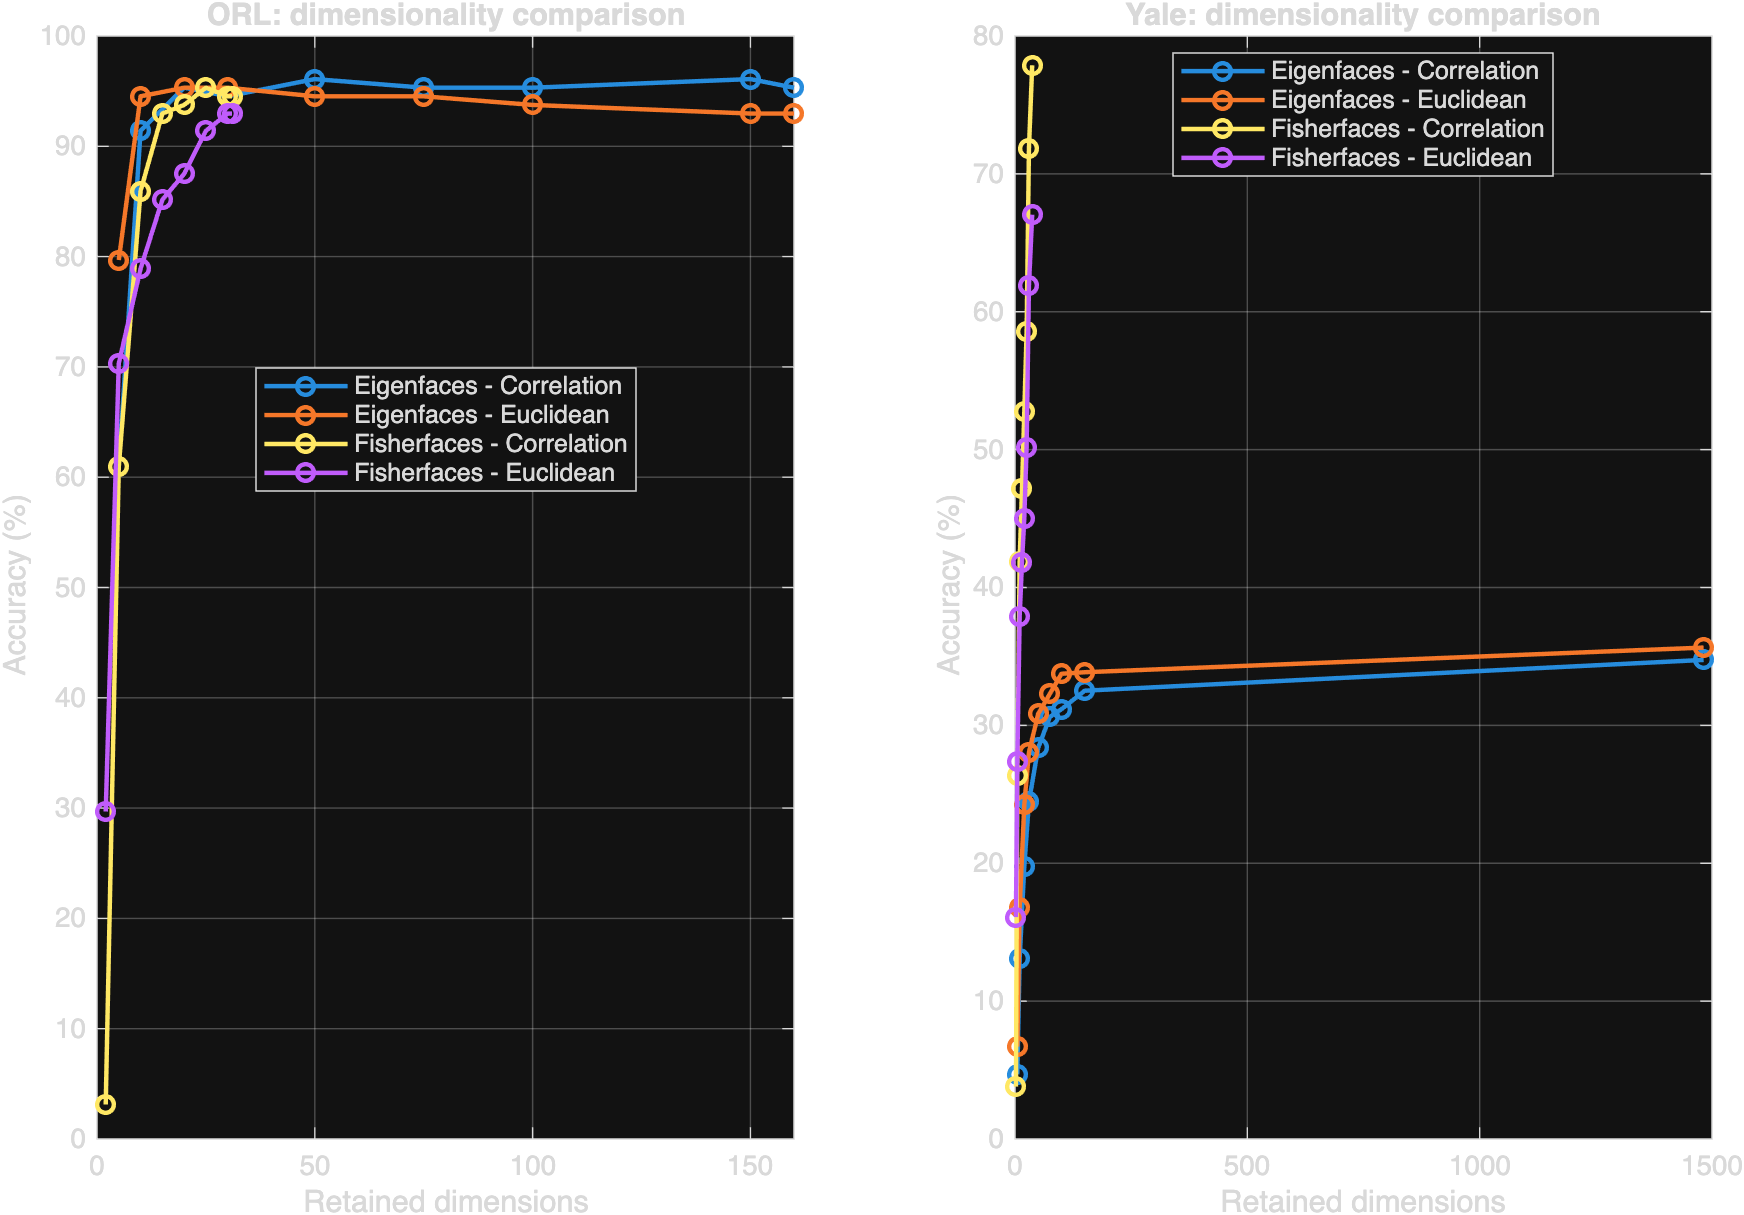
\includegraphics[width=\linewidth]{figures/accuracy_vs_dimensions.png}
\caption{Accuracy as the number of retained dimensions changes.}
\end{minipage}\hfill
\begin{minipage}[t]{0.48\textwidth}\centering
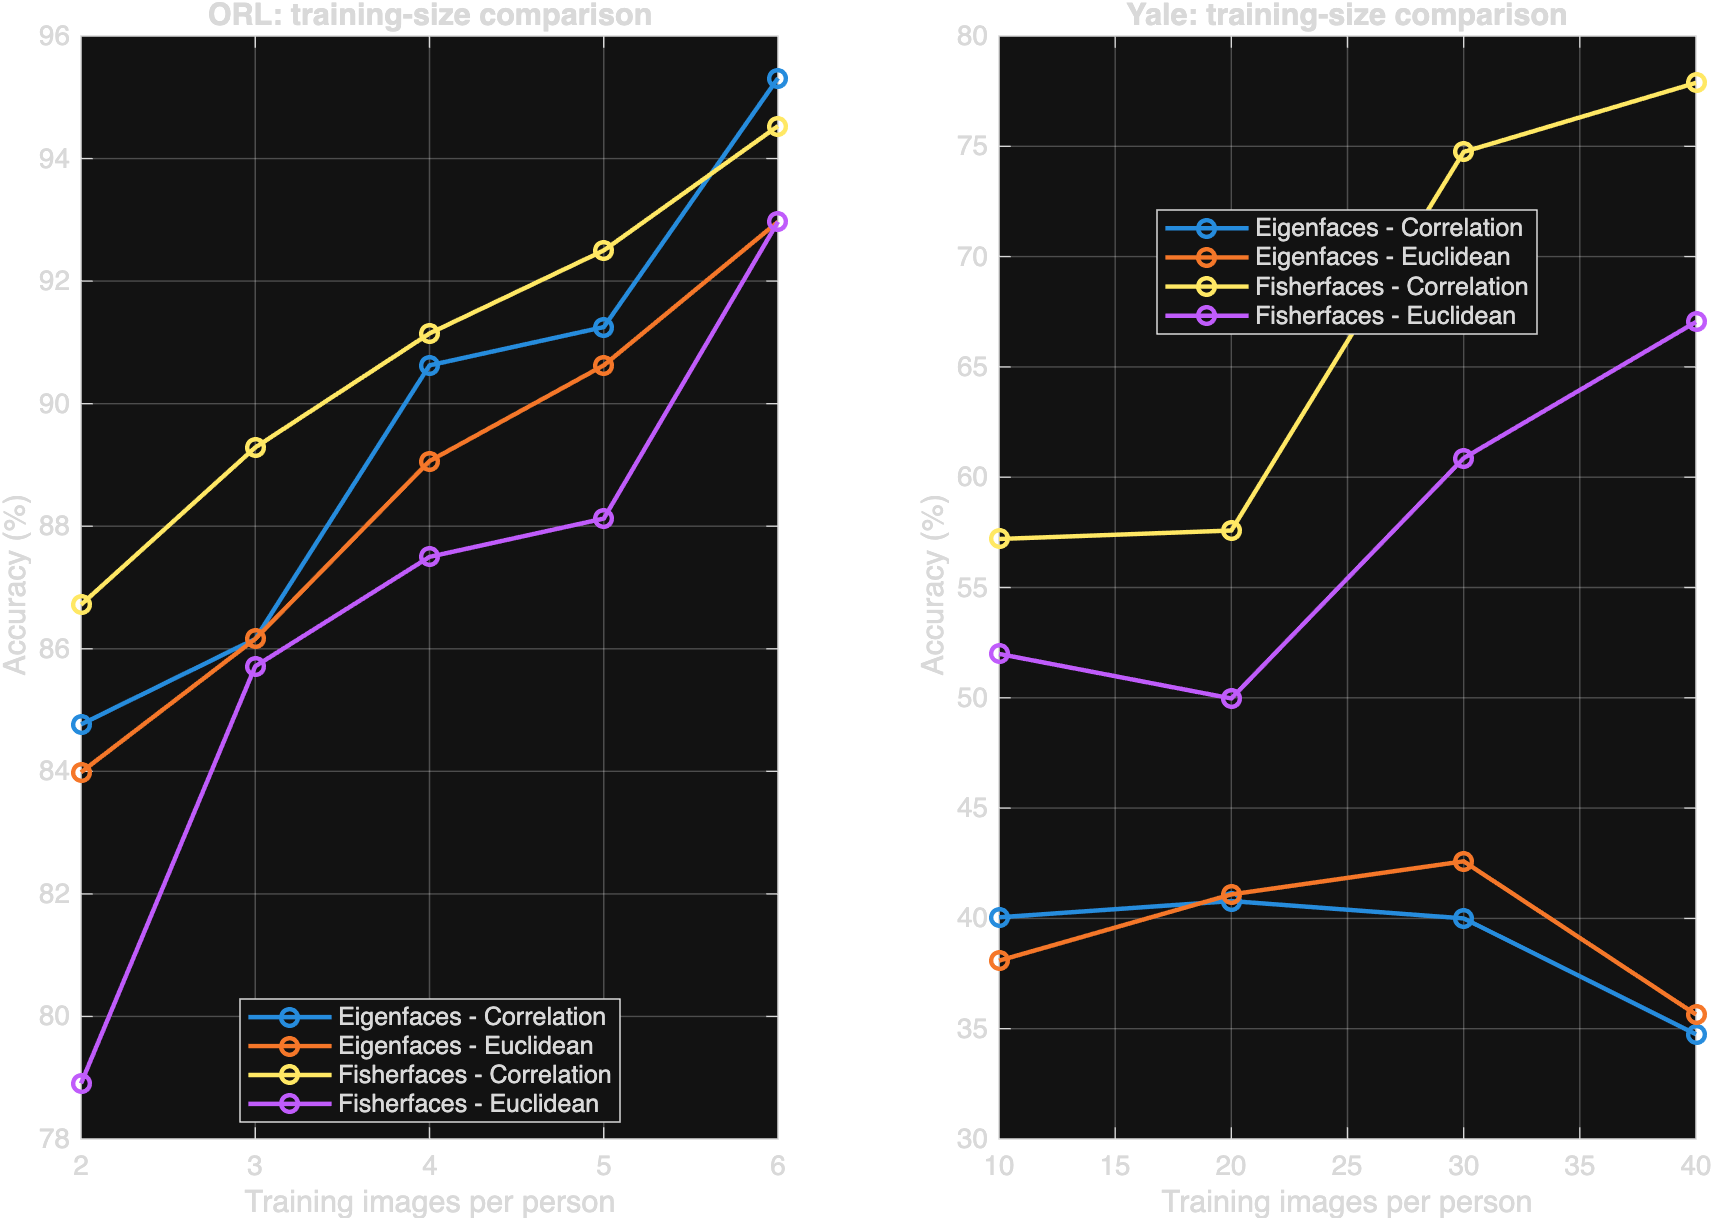
\includegraphics[width=\linewidth]{figures/accuracy_vs_training_images.png}
\caption{Accuracy as the number of training images per subject changes.}
\end{minipage}
\end{figure}

On ORL, Eigenfaces reaches its best correlation accuracy of 96.09\% at 50 retained dimensions. Fisherfaces reaches 95.31\% at 25 dimensions, showing that it needs fewer discriminant coordinates. On Yale, Eigenfaces peaks at only 35.64\%, whereas Fisherfaces reaches 77.88\% using 37 FLD dimensions.

\clearpage
\section{PCA Visualization}
\begin{figure}[h!]
\centering
\begin{minipage}[t]{0.48\textwidth}\centering
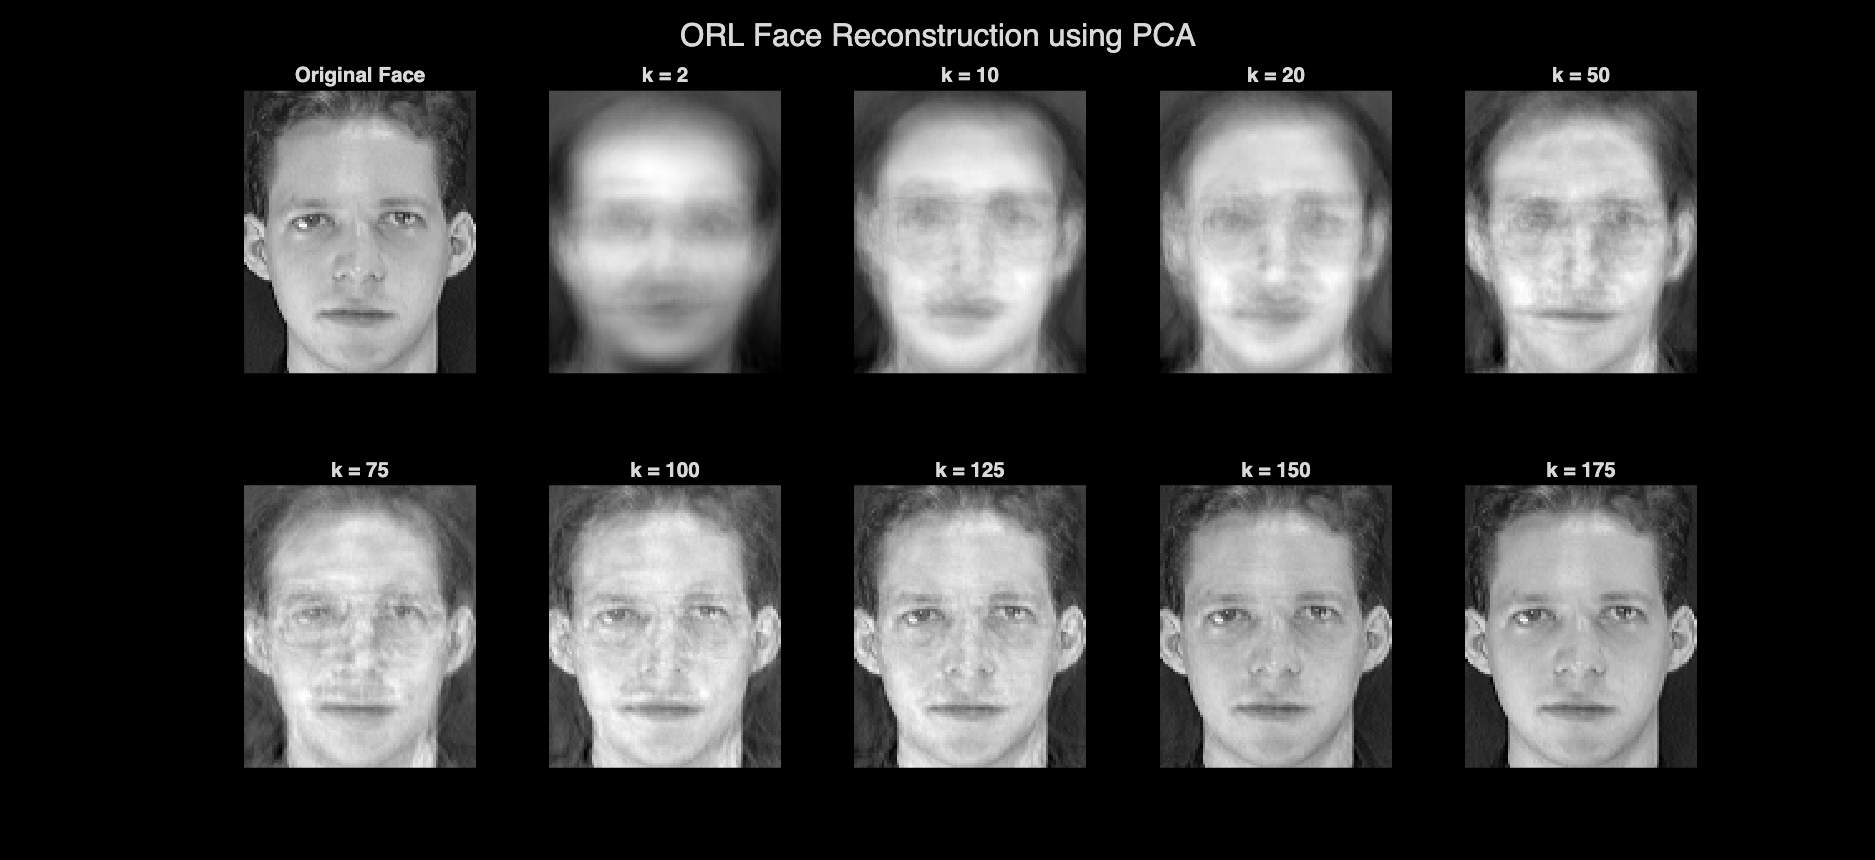
\includegraphics[width=\linewidth]{figures/orl_reconstruction.png}
\caption{Results of reconstruction: $k=2,10,20,50,75,100,125,150$, and $175$.}
\end{minipage}\hfill
\begin{minipage}[t]{0.48\textwidth}\centering
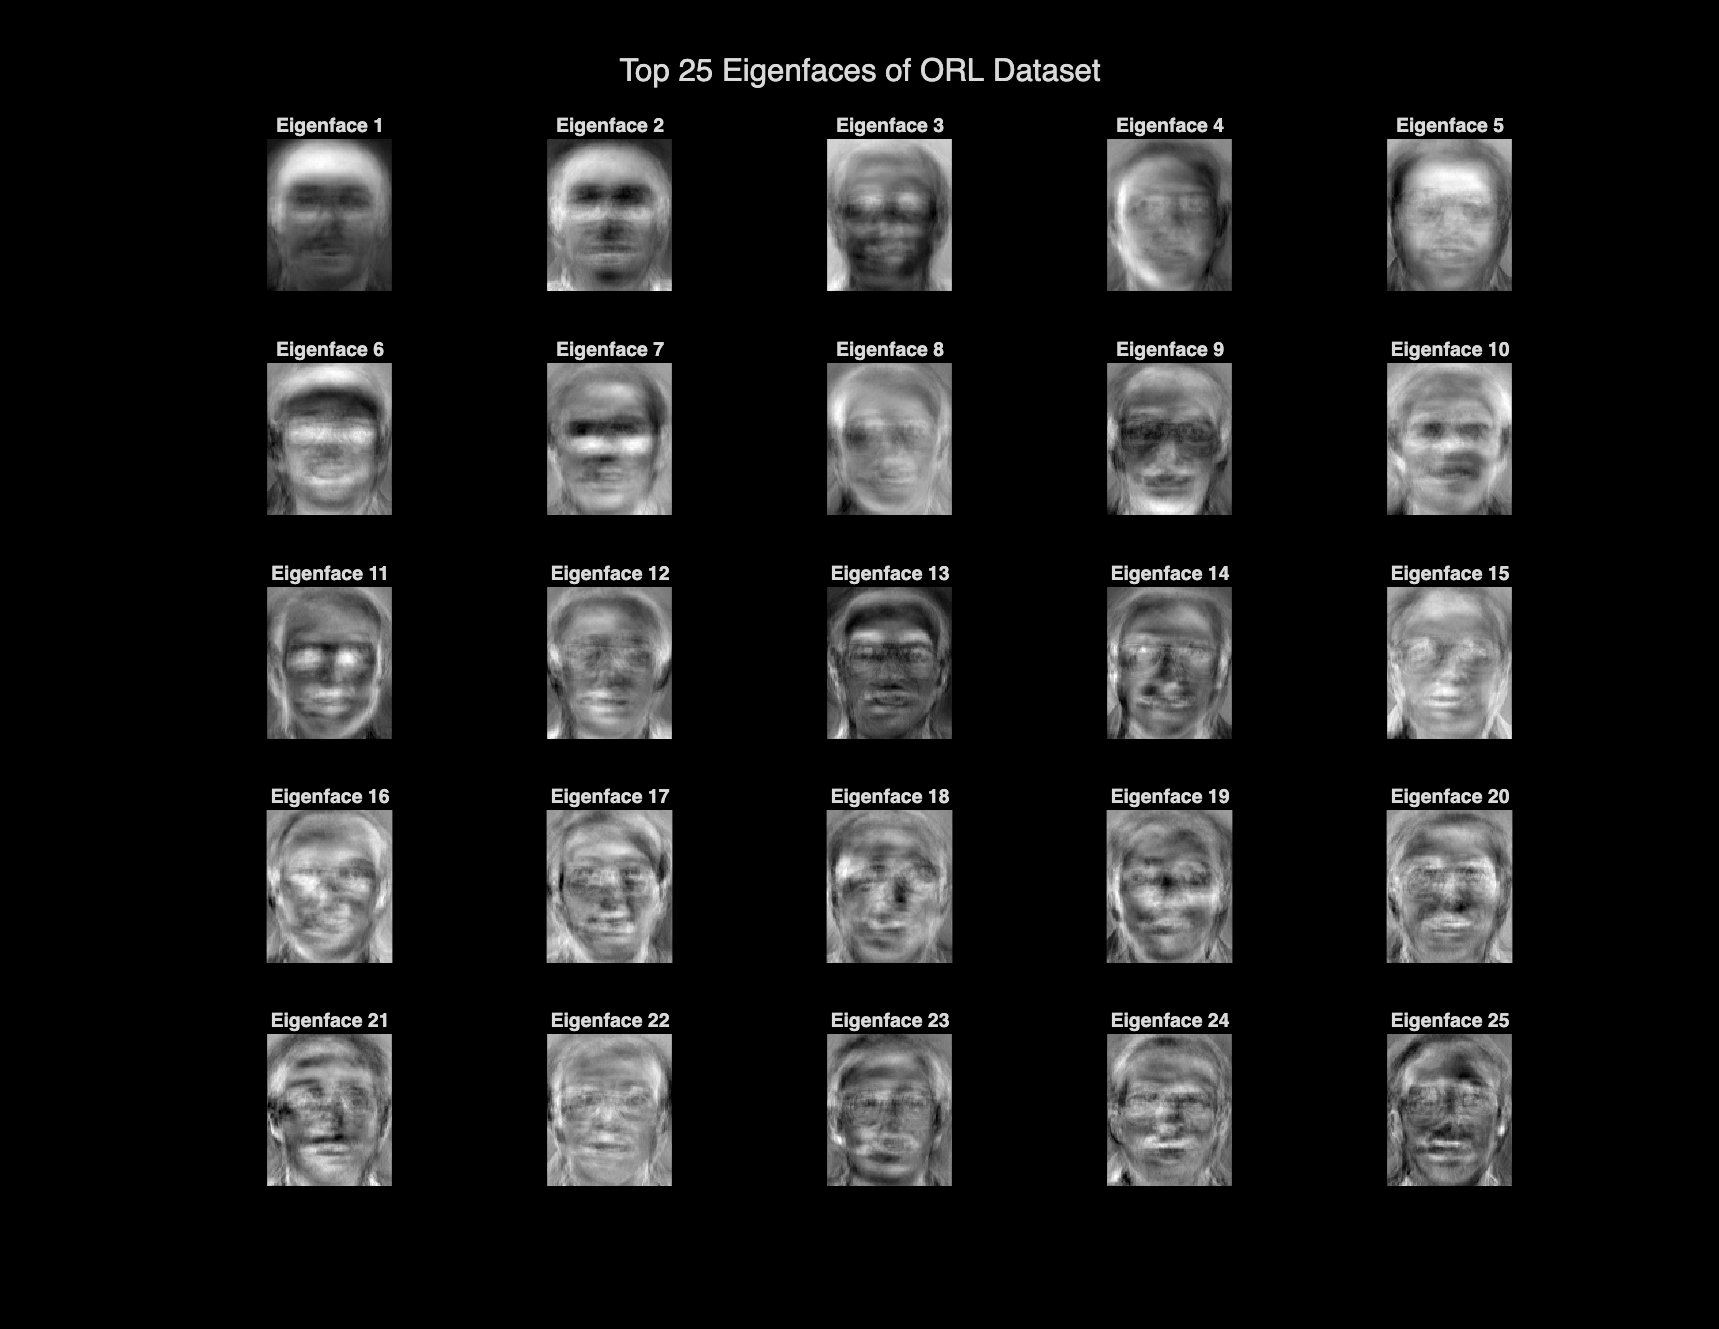
\includegraphics[width=\linewidth]{figures/orl_top25_eigenfaces.png}
\caption{First 25 ORL eigenfaces.}
\end{minipage}
\end{figure}

\section{4. Visual Recognition Examples}
The following examples show a probe image and its nearest Fisherface gallery match. In both cases the predicted identity is subject 1. The Yale example is more challenging because the two images have very different illumination.

\begin{figure}[h!]
\centering
\begin{minipage}[t]{0.48\textwidth}\centering
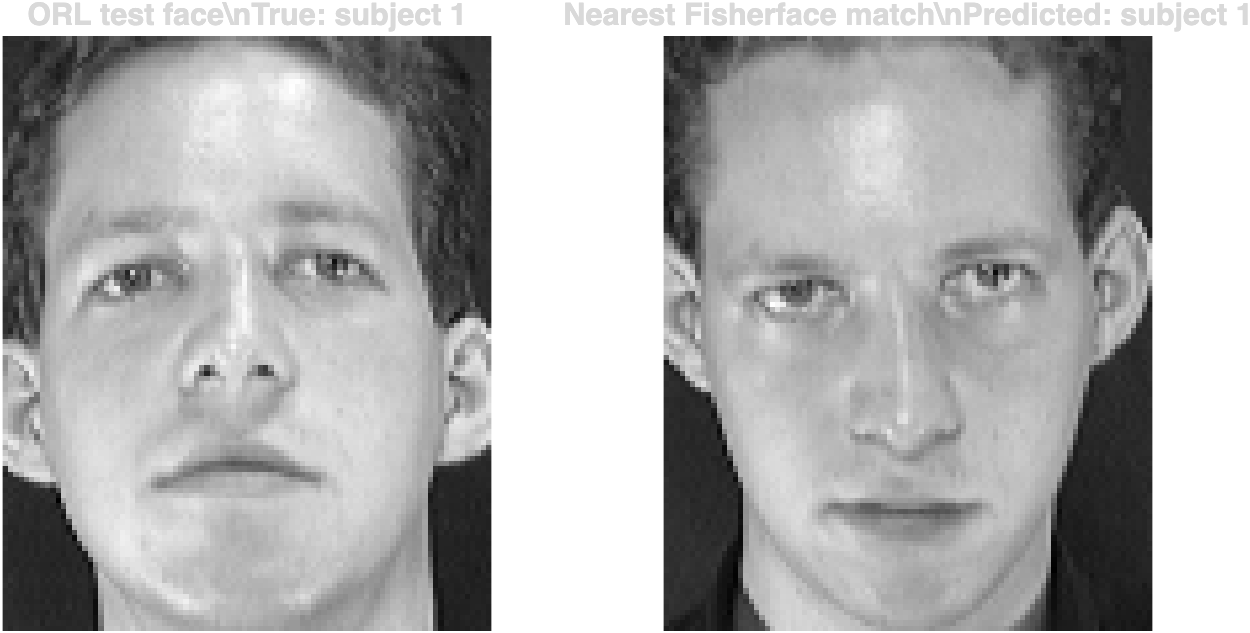
\includegraphics[width=\linewidth]{figures/orl_fisherfaces_demo.png}
\caption{ORL: probe face and nearest Fisherface match.}
\end{minipage}\hfill
\begin{minipage}[t]{0.48\textwidth}\centering
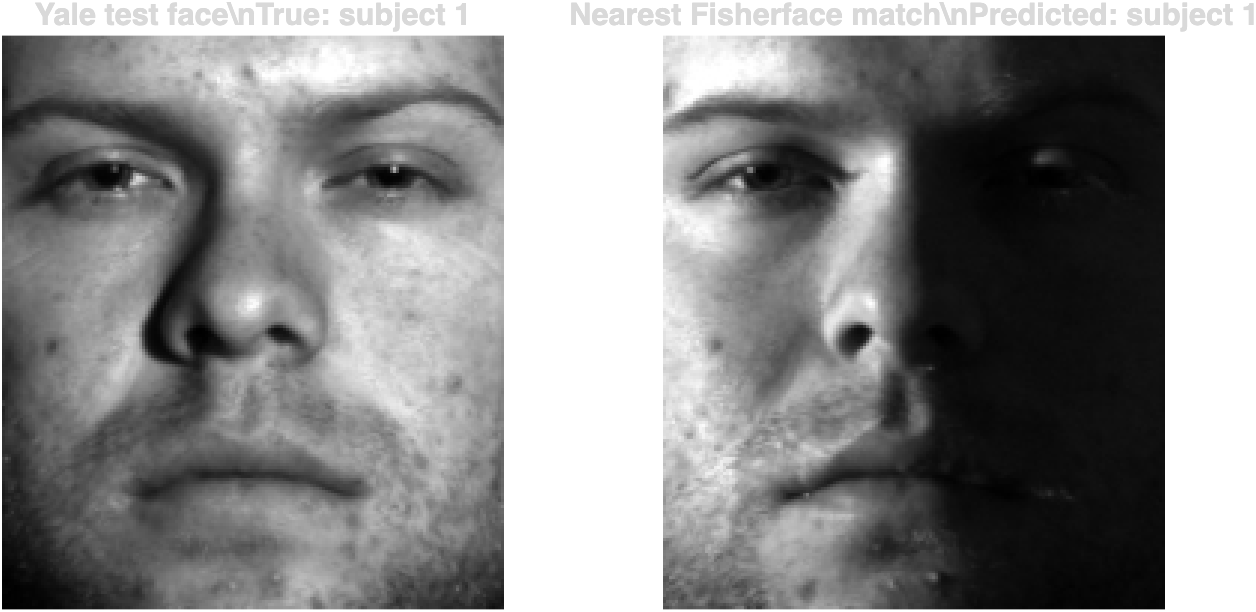
\includegraphics[width=\linewidth]{figures/yale_fisherfaces_demo.png}
\caption{Yale: probe face and nearest Fisherface match.}
\end{minipage}
\end{figure}

\section{Code Link}
Project source code:\newline
\url{https://github.com/yashwanthsudi10/CS_740_Project}

\section{5. Conclusion}
The implementation confirms the main message of the paper. PCA/Eigenfaces is a strong compact baseline when conditions are controlled, as seen on ORL. However, PCA retains directions of total image variation, including lighting variation that does not identify a person. Fisherfaces uses class labels through FLD and produces a much more discriminative representation under Yale's severe illumination changes. The final Yale result, 77.88\% with Fisherfaces and correlation matching versus 35.64\% for the best Eigenfaces setting, demonstrates this advantage clearly.

\section{References}
\begin{enumerate}
\item P. N. Belhumeur, J. P. Hespanha, and D. J. Kriegman, ``Eigenfaces vs. Fisherfaces: Recognition Using Class Specific Linear Projection,'' \textit{IEEE Transactions on Pattern Analysis and Machine Intelligence}, vol. 19, no. 7, pp. 711--720, 1997.
\item ``Mod-06 Lec-17: Fisher Linear Discriminant,'' YouTube Lecture. \url{https://youtu.be/9K5NL4nfi0Y}
\end{enumerate}
\end{document}
